% $Id: perspectives.tex 12369 2010-09-28 08:34:59Z markus $
% Local Variables:
% ispell-check-comments: nil
% Local IspellDict: american
% End:
% --------------------------------------------------------
% User documentation
% copyright by BREDEX GmbH 2004
% --------------------------------------------------------
\index{Perspective!Execution}
\index{Execution!Perspective}
\index{View!Test Result}
\index{Test Result!View}

There are five perspectives in \app{}: 
\begin{itemize}
\item Specification
\gdmarpar{../../../share/PS/perspectivesp}{specification}
 \item Execution
\gdmarpar{../../../share/PS/perspectiveex}{execution}
\item Modeling
%\gdmarpar{../../../share/PS/perspectiveex}{execution}
\item Workspace
\item Reporting

\end{itemize} 


\subsection{The specification perspective}
\index{Specification!Perspective}
\index{Perspective!Specification}
\index{Browser!Test Suite}
\index{Browser!Test Case}
\index{Browser!Component Name}
\index{View!Editor}
\index{View!Properties}
\index{View!Data Sets}
\index{View!Problem}
\index{Test Suite!Browser}
\index{Test Case!Browser}
\index{Component Name Browser}
\index{Editor!View}
\index{Properties View}
\index{Data Sets View}
\index{Problem View}
\index{Component!Names!View}
\index{View!Component Names}
The specification perspective (\bxfigref{clientwindow}) provides browsers, editors and views to let you create tests. It contains:

\begin{itemize}
\item The \gdtestsuitebrowser{} 
\item The \gdtestcasebrowser{} 
\item The \gdcompnamebrowser{} 
\item The editor area 
\item The \gdpropview{} 
\item The \gddatasetsview{} 
\item The \gdcompnamesview{} 
\item The \gdprobview{} 
\item The search result view (behind the \gdprobview{})
\item The \gdrunautview{}
\end{itemize}

\begin{figure}
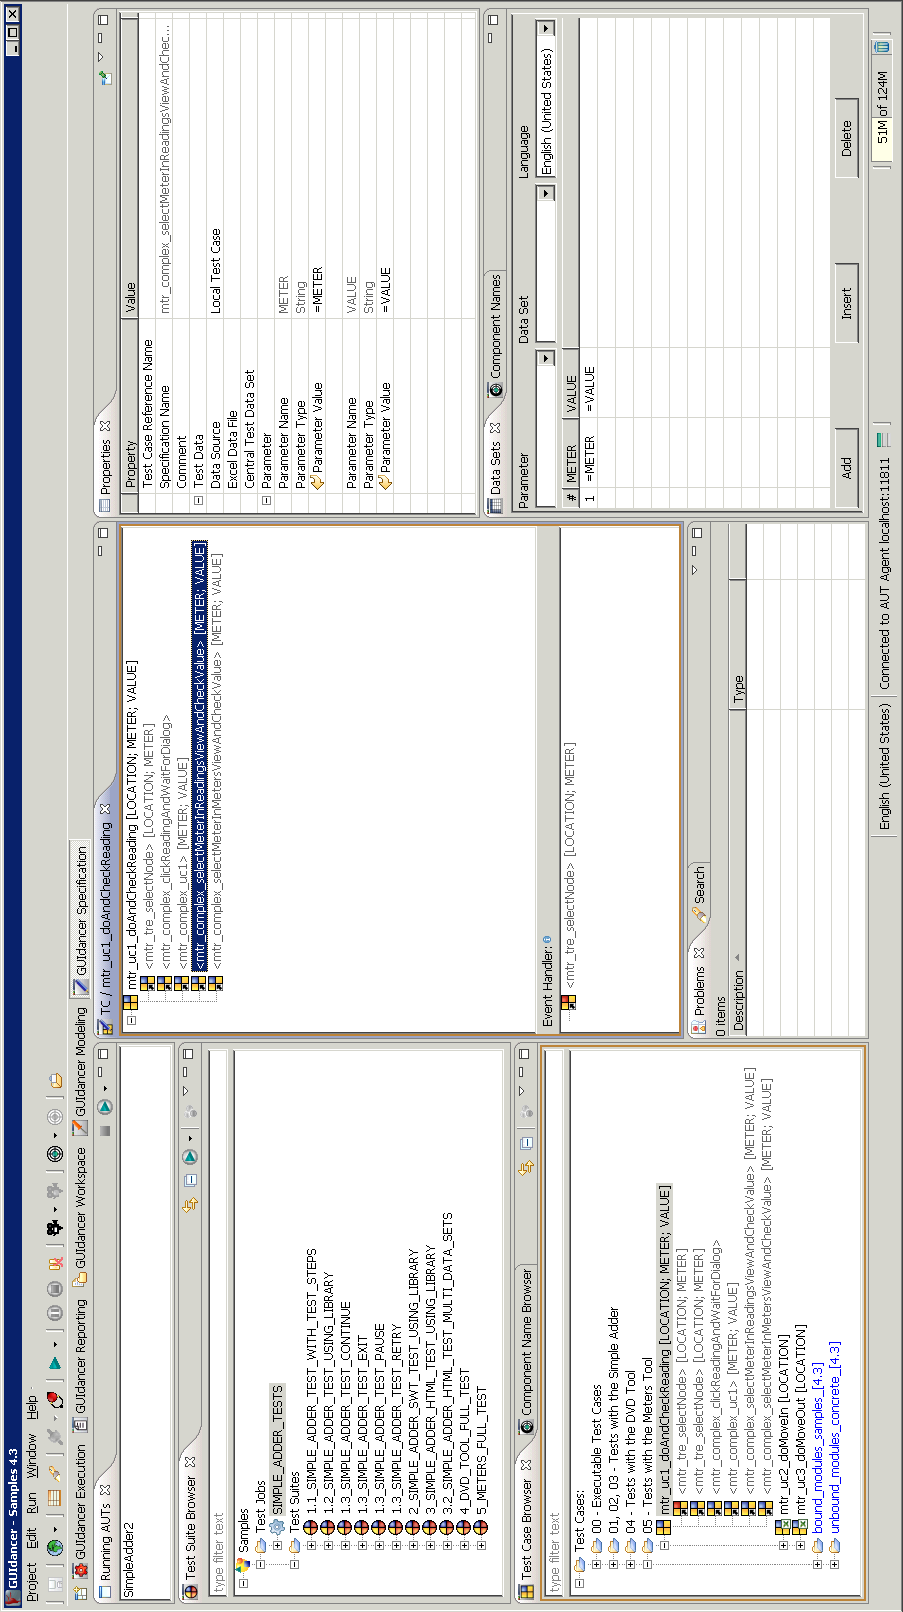
\includegraphics[width=12.5cm]{Userinterface/Editors/PS/client}
\caption{\app{} Specification Perspective}
\label{clientwindow}
\end{figure}

\clearpage

The \gdtestcasebrowser{} and the \gdtestsuitebrowser{} let you see your \gdcases{} and \gdsuites{}. If you double-click an item in one of these browsers, an editor for this item opens. Using the editor and its support views (numbers 4-6) you can edit the contents and properties of \gdsuites{}, \gdcases{} and \gdsteps{}. The content of the support view changes according to the currently selected item. 
 \clearpage
\subsection{The execution perspective}
\index{Execution!Perspective}
\index{Perspective!Execution}
\index{Views!Test Result}
\index{Test Result!View}

In the execution perspective, you can see the following (\bxfigref{executionclient}):


\begin{itemize}
\item \gdtestsuitebrowser 
\item \gdtestresultview 
\item \gdpropview 
\item \gddatasetsview
\end{itemize}


\begin{figure}
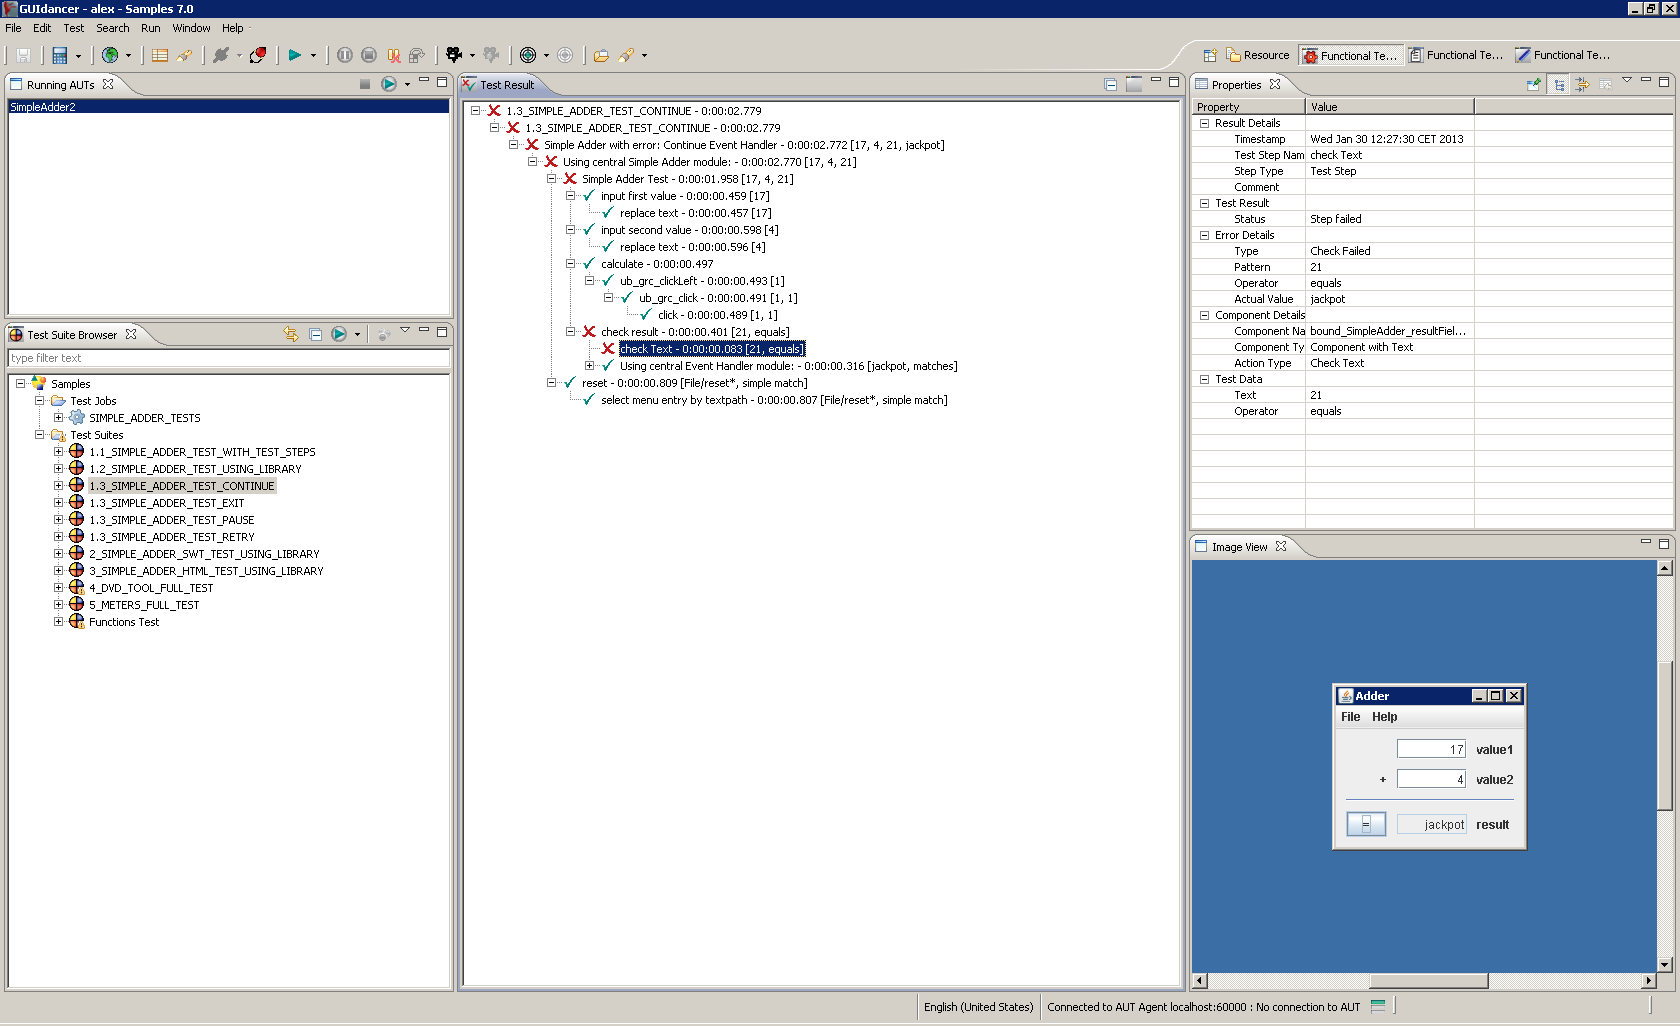
\includegraphics{Userinterface/Editors/PS/executionclient}
\caption{\app{} Execution Perspective}
\label{executionclient}
\end{figure}

You cannot edit in the execution perspective, but you can see your \gdsuite{} and its results. 
\clearpage

\subsection{The modeling perspective}
\index{Perspective!Modeling}
\index{Modeling!Perspective}
\index{Views!Navigator}
\index{Navigator View}
\index{Outline View}
\index{Views!Outline}
\index{Editor!Test Case Model}
\index{Test Case!Model Editor}

In the modeling perspective (\bxfigref{modelperspective}), you can create \gdprojects{} in your workspace to create and import model diagrams which can then be generated into a \gdcase{\ structure. The modeling perspective contains the following:


\begin{itemize}
\item \gdnavview{} 
\item \gdmodeleditor{}
\item \bxname{Outline View}
\item \gdpropview{}
\item \bxname{Console}
\item \gdtestcasebrowser{}
\item \gdprobview{}
\end{itemize}

\begin{figure}
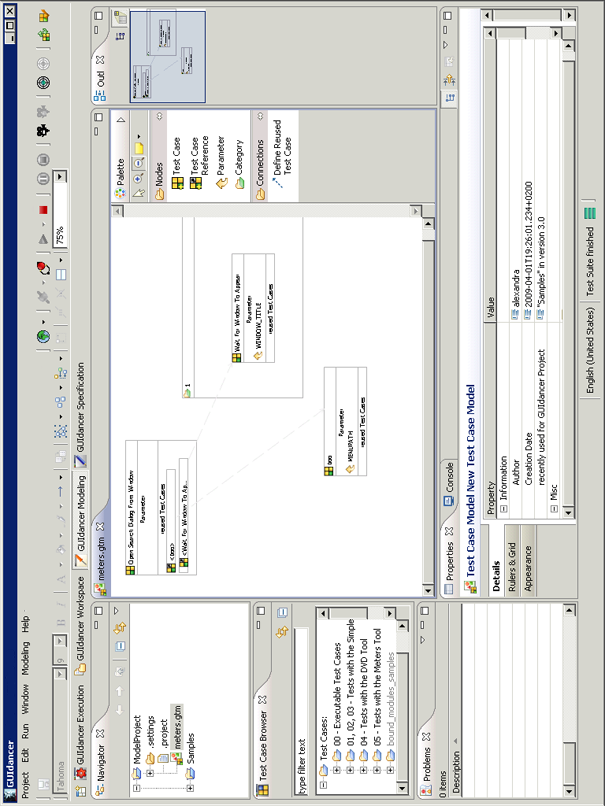
\includegraphics{Userinterface/Editors/PS/modelperspective}
\caption{\app{} Modeling Perspective}
\label{modelperspective}
\end{figure}

\clearpage

\subsection{The \app{} workspace perspective}
\index{Perspective!Workspace}
\index{Workspace!Perspective}
\index{Views!Navigator}
\index{Navigator View}


In the workspace perspective (\bxfigref{workspaceperspective}), you can view the \gdprojects{} and files in your \app{} workspace. The workspace perspective contains the following:


\begin{itemize}
\item \gdnavview{} 
\item An editor area to view e.g. Excel and HTML files.
\end{itemize}

\begin{figure}
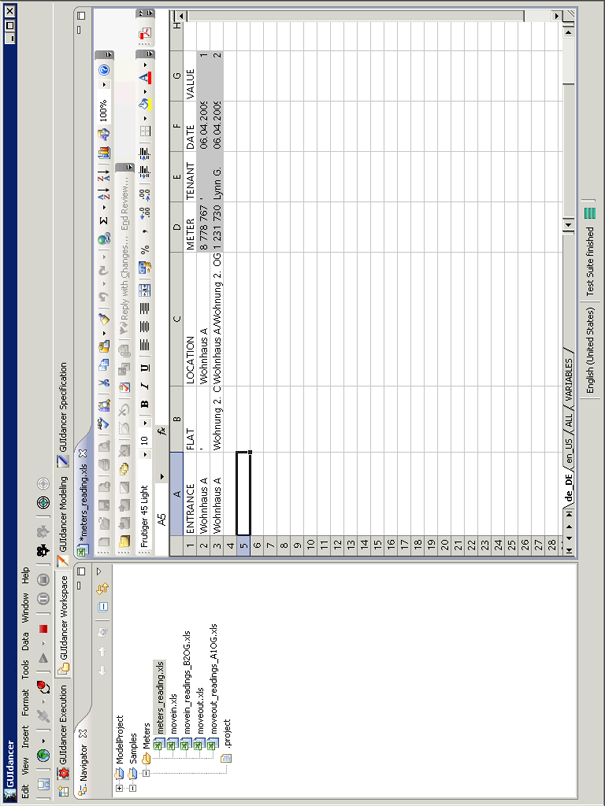
\includegraphics{Userinterface/Editors/PS/workspaceperspective}
\caption{\app{} Workspace Perspective}
\label{workspaceperspective}
\end{figure}
\clearpage

\subsection{The \app{} reporting perspective}
\index{Perspective!Reporting}
\index{Reporting!Perspective}
\index{Views!Test Result Summary}
\index{Test Result Summary View}
In the reporting perspective, the only view is the \gdtestsummaryview{}. You can see an overview of all tests that have run in this \gddb{}.

\begin{figure}
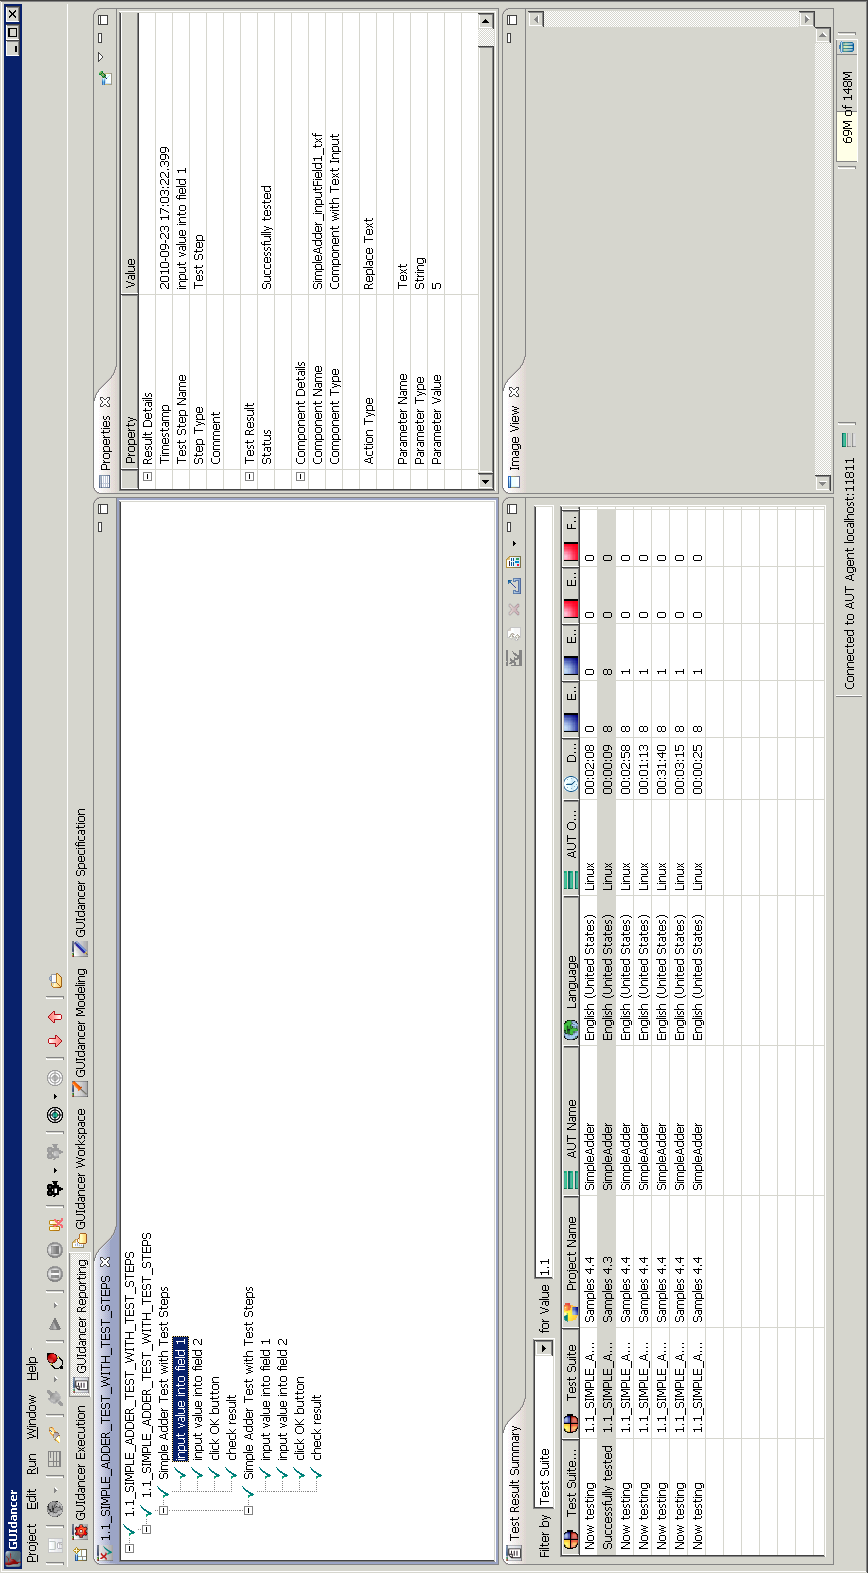
\includegraphics[width=12.5cm]{Userinterface/Editors/PS/reportingperspective}
\caption{\app{} Reporting Perspective}
\label{reportingperspective}
\end{figure}
\clearpage
